\documentclass{beamer}

\mode<presentation>
{
  \usetheme{Goettingen}      
  \usecolortheme{default}
  \usefonttheme{default}
  \setbeamertemplate{navigation symbols}{}
  \setbeamertemplate{caption}[numbered]
} 

\usepackage[english]{babel}
\usepackage[utf8x]{inputenc}
\usepackage{amsmath}
\usepackage{dsfont}
\usepackage{booktabs,multirow,array}
\usepackage{algorithm}
\usepackage{caption}
\usepackage{subcaption}
\usepackage{graphicx}
\usepackage{url}
\usepackage{xcolor}
\usepackage{moresize}
\usepackage{lmodern}
\usepackage{mathrsfs}

\usepackage[numbers]{natbib}
\renewcommand\bibsection{\section[]{\refname}}

\definecolor{blue_pres}{RGB}{51,50,178}
\definecolor{darkpastelgreen}{rgb}{0.01, 0.75, 0.24}

\hypersetup{
    colorlinks,
    citecolor=orange,
    linkcolor=blue_pres,
    backref=true,
    urlcolor=darkpastelgreen
}

\makeatletter
\let\@@magyar@captionfix\relax
\makeatother

\DeclareCaptionFormat{myformat}{#3}
\captionsetup[algorithm]{format=myformat}
\usepackage{algpseudocode}

%%%%%%%%%%%%%%%%%%%%
%%% New commands %%%
%%%%%%%%%%%%%%%%%%%%

\DeclareMathOperator{\TV}{TV}
\DeclareMathOperator{\bina}{bina}
\DeclareMathOperator{\argmin}{argmin}

\newcommand{\dd}{\mathrm{d}}
\newcommand{\bC}{\mathbb C}
\newcommand{\bD}{\mathbb D}
\newcommand{\bP}{\mathbb P}
\newcommand{\bX}{\boldsymbol X}
\newcommand{\XB}{{\boldsymbol X}^B}
\newcommand{\E}{\mathbb E}
\newcommand{\N}{\mathbb N}
\newcommand{\bigO}{\mathcal{O}}
\newcommand{\C}{\mathbb{C}}
\newcommand{\D}{\mathbb{D}}
\newcommand{\R}{\mathbb R}
\newcommand{\cA}{\mathcal A}
\newcommand{\cB}{\mathcal B}
\newcommand{\cH}{\mathcal H}
\newcommand{\cS}{\mathcal S}
\newcommand{\cM}{\mathcal M}
\newcommand{\cC}{\mathcal C}
\newcommand{\cG}{\mathcal G}
\newcommand{\cN}{\mathcal N}
\newcommand{\cU}{\mathcal U}
\renewcommand{\P}{\mathds{P}}
\newcommand{\Gb}{\bar G}
\newcommand{\Fb}{\bar F}
\newcommand{\Ub}{\bar U}
\newcommand{\by}{\boldsymbol y}
\newcommand{\bz}{\boldsymbol z}
\newcommand{\bdelta}{\boldsymbol \delta}
\newcommand{\bSigma}{\textbf{$\Sigma$}}
\newcommand{\norm}[1]{\|#1\|}
\newcommand{\pluseq}{\mathrel{+}=}
\newcommand{\minuseq}{\mathrel{-}=}
\newcommand{\bcdot}{\raisebox{-0.25ex}{\scalebox{1.2}{$\cdot$}}}
\newcommand{\ind}[1]{\mathds{1}_{#1}}
\newcommand\independent{\protect\mathpalette{\protect\independenT}{\perp}} 
\newcommand{\cD}{\mathcal D}
\newcommand{\cQ}{\mathcal Q}
\newcommand{\cR}{\mathcal R}
\renewcommand{\P}{\mathds P}


\definecolor{blue_pres}{RGB}{51,50,178}

\newcommand\Algphase[1]{%
\vspace*{-.7\baselineskip}\Statex\hspace*{\dimexpr-\algorithmicindent-2pt\relax}\rule{\textwidth}{0.4pt}%
\vspace*{-.4\baselineskip}\Statex\hspace*{\algorithmicindent}\textbf{#1}%
\vspace*{-.7\baselineskip}\Statex\hspace*{\dimexpr-\algorithmicindent-2pt\relax}\rule{\textwidth}{0.4pt}%
}
\newcommand*\rot{\rotatebox{90}}
\newcommand*\OK{\ding{51}}

\def\independenT#1#2{\mathrel{\rlap{$#1#2$}\mkern2mu{#1#2}}}
\newtheorem{hyp}{Hypothesis}

\begin{document}

\section{Introduction}

\begin{frame}[noframenumbering]
\Large \centering
\textcolor{blue_pres}{I.} Introduction
\end{frame}

\subsection{Overview}

\begin{frame}{Overview}

\begin{itemize}
  \item Deal with the problem of joint modeling of longitudinal data and censored durations
  \item Large number of both longitudinal and time-independent features are available
  \item Flexibility in modeling the dependency between the longitudinal features and the event time with appropriate penalties
  \item Inference achieved using an efficient and novel Quasi-Newton Monte Carlo Expectation Maximization algorithm
\end{itemize}

\end{frame}

\subsection{Use cases}

\begin{frame}{Use cases}

\small
\begin{itemize}
  \item Predict the risk for an event of interest to occur quickly, taking into account simultaneously a huge number of longitudinal signals in a high-dimensional context
  \item Provides powerful interpretability by automatically pinpointing significant time-dependent and time-independent features
\end{itemize}

\begin{block}{Real-time decision support}
\begin{itemize}
  \item Medical context $\rightarrow$ event of interest: survival time, re-hospitalization, relapse or disease progression ; longitudinal data: biomarkers or vital parameters measurements
  \item Customer's satisfaction monitoring context $\rightarrow$ event of interest: time when a client churns ; longitudinal data: the client's activity recorded from account opening throughout the duration of the business relationship
\end{itemize}
\end{block}

\end{frame}

\subsection{Framework}

\begin{frame}{High-dimensional framework}

\small
\begin{itemize}
  \item Survival analysis
  \begin{center}
  $T = T^\star \wedge C \quad \text{and} \quad \Delta = \ind{\{T^\star \leq C\}}$
  \end{center}
  \item Time-independent features $X \in \R^p$ with $p \gg n$
  \item $L$ longitudinal outcomes such that $L \gg n$ and \[Y(t) = \big(Y^1(t), \ldots, Y^L(t) \big)^\top \in \R^L\]
  \item Heterogeneity of the population: latent subgroups \[G \in \{ 0, \ldots, K-1\}\]
  \item Softmax link function for the latent class membership probability given time-independent features
  \begin{center}
  $\pi_{\xi_k}(x) = \P[G=k|X=x] = \dfrac{e^{x^\top\xi_k}}{\sum_{k=0}^{K-1}e^{x^\top\xi_k}}$
  \end{center}
\end{itemize}

\end{frame}

\section{Model}

\begin{frame}[noframenumbering]
\Large \centering
\textcolor{blue_pres}{II.} Model
\end{frame}

\subsection{Submodels}

\begin{frame}{Submodels}

\small
\begin{block}{Group-specific marker trajectories}
\begin{itemize}
  \item \footnotesize $h_l\big(\E[Y^l(t)|b^l, G=k]\big) = m_k^l(t) = u^l(t)^\top\beta_k^l + v^l(t)^\top b^l$\\
  with fixed effect parameters $\beta_k^l \in \R^{q_l}$ and subject-and-longitudinal outcome specific random effects $b^l \in \R^{r_l} \sim \cN(0, D_{ll})$
  \item $\text{Cov}[b^l,b^{l'}] = D_{ll'}$
  \only{ and
  \[ D = 
  \begin{bmatrix}
    D_{11} & \cdots & D_{1L}\\
    \vdots &  \ddots & \vdots \\
    D_{1L}^\top & \cdots & D_{LL}
  \end{bmatrix}
  \]
  the global variance-covariance matrix}

\end{itemize}
\end{block}

\end{frame}

\begin{frame}{Submodels}

\small
\begin{block}{Group-specific risk of event}
\begin{itemize}
  \item \footnotesize $\lambda(t|G = k) = \lambda_0(t) \exp \Big\{ \sum_{l=1}^L \sum_{a=1}^\cA {\gamma_{k,a}^l}^\top \varphi_{k, a}(t, b^l) \Big\}$
  \item Functionals $(\varphi_a)_{a\in \cA}$
\begin{table}[htb]
\centering
\resizebox{.9\textwidth}{!}{%
\begin{tabular}{ccccc}
\toprule
Description & $\varphi_{k,a}(t, b^l)$ & $\imath_a$ & Reference \\
\midrule
Linear predictor & $m_k^l(t)$ & 1 & \citet{chi2006joint} \\ [.15cm]
Random effects & $b^l$ & $r_l$ & \citet{hatfield2011joint} \\
Time-dependent slope & $\dfrac{\dd}{\dd t} m_k^l(t)$ & 1 & \citet{rizopoulos2011bayesian} \\ [.3cm]
Cumulative effect & $\int_0^t m_k^l(s) \dd s$ & 1 & \citet{andrinopoulou2017combined} \\ [.1cm]
 \bottomrule
\end{tabular}}
\end{table}

\end{itemize}
\end{block}

\end{frame}

\begin{frame}{Submodels}
\begin{itemize}
\item Graphical representation of a joint model of a time-to-event submodel and K-multivariate longitudinal outcomes submodel
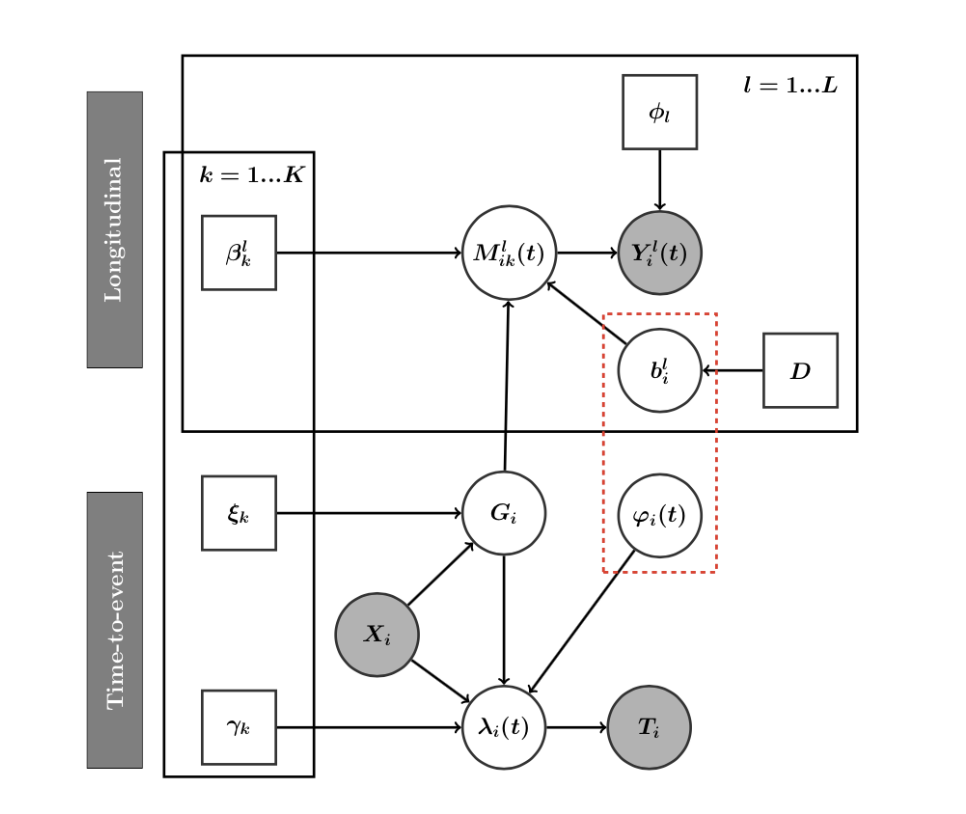
\includegraphics[scale=0.42]{figures/lights_graphical_representation.png}
\end{itemize}

\end{frame}
\subsection{Notations}

\begin{frame}{Notations}

\footnotesize
\begin{itemize}
  \item $\cD_n = \big\{ (x_1, y_1^1, \ldots, y_1^L, t_1, \delta_1), \ldots, (x_n, y_n^1, \ldots, y_n^L, t_n, \delta_n) \big\}$ with $y_i^l=(y_{i1}^l, \ldots, y_{in_i^l}^l)^\top \in \R^{n_i^l} \text{ and } y_{ij}^l=Y_i^l(t_{ij}^l)$
  \item $y_i = ({y_i^1}^\top \cdots {y_i^L}^\top)^\top \in \R^{n_i}$ with $n_i = \sum_{l=1}^L n_i^l$
  \item $b_i = ({b_i^1}^\top \cdots {b_i^L}^\top)^\top \in \R^r$ with $r = \sum_{l=1}^L r_l$
  \item Design matrices
  \[ U_i = 
\begin{bmatrix}
  U_{i1} & \cdots & 0\\
  \vdots &  \ddots & \vdots \\
  0 & \cdots & U_{iL}
\end{bmatrix} 
\in \R^{n_i \times q}
\text{ and }
V_i = 
\begin{bmatrix}
  V_{i1} & \cdots & 0\\
  \vdots &  \ddots & \vdots \\
  0 & \cdots & V_{iL}
\end{bmatrix}
\in \R^{n_i \times r}
\]
with $q = \sum_{l=1}^L q_l$ and where for all $l=1, \ldots, L$, one writes
\[
\left\{
    \begin{array}{ll}
        U_{il} &= \big(u_i^l(t_{i1}^l)^\top \cdots u_i^l(t_{in_i^l}^l)^\top\big)^\top \in \R^{n_i^l \times q_l},\\
        V_{il} &= \big(v_i^l(t_{i1}^l)^\top \cdots v_i^l(t_{in_i^l}^l)^\top\big)^\top \in \R^{n_i^l \times r_l}.
    \end{array}
\right.
\]
  \item $\beta_k = ({\beta_k^1}^\top \cdots {\beta_k^L}^\top)^\top \in \R^q$
  \item $M_{ik} = U_i\beta_k + V_ib_i \in \R^{n_i}$
\end{itemize}

\end{frame}

\subsection{Likelihood}

\begin{frame}{Likelihood}

\footnotesize
\begin{itemize}
  \item \scriptsize $\theta = \big(\xi_0^\top \cdots \xi_{K-1}^\top, \beta_0^\top \cdots \beta_{K-1}^\top, \phi^\top, \text{vech}(D), \lambda_0^\top, \gamma_0^\top \cdots \gamma_{K-1}^\top\big) \in \R^\vartheta$
  \item $f(y_i|b_i, G_i=k) = \exp \big\{(y_i \odot \Phi_i)^\top M_{ik} - c_\phi(M_{ik}) + d_\phi(y_i) \big\}$ with $\Phi_i = (\phi_1^{-1} {\textbf{1}_{n_i^1}}^\top \cdots \phi_L^{-1} {\textbf{1}_{n_i^L}}^\top)^\top \in \R^{n_i}$
  \item Survival part:
  \begin{align*}f(t_i, \delta_i| b_i, G_i = k ; \theta) = &\big[\lambda(t_i|\cM_k(t_i), G_i = k)\big]^{\delta_i} \\ & \times \exp \Big\{-\int_0^{t_i} \lambda(s|\cM_k(s), G_i = k) \dd s \Big\}
  \end{align*}
  \item Then, the likelihood writes
  \begin{align*}\ell_n(\theta) = n^{-1} \sum_{i=1}^n \log \int_{\R^r} \sum_{k=0}^{K-1} &\pi_{\xi_k}(x_i) f(t_i, \delta_i| b_i, G_i = k ; \theta) \\ & \times f(y_i | b_i, G_i = k ; \theta) f(b_i ; \theta) \dd b_i
  \end{align*}
\end{itemize}

\end{frame}

\section{Inference}

\begin{frame}[noframenumbering]
\Large \centering
\textcolor{blue_pres}{III.} Inference
\end{frame}

\subsection{Penalization}

\begin{frame}{Penalization}

\small

\begin{itemize}
  \item Penalized objective
  \begin{equation*}
  \ell_n^\text{pen}(\theta) = - \ell_n(\theta) + \sum_{k=0}^{K-1} \zeta_{1,k} \norm{\xi_k}_{\text{en}, \eta} + \zeta_{2,k} \norm{\gamma_k}_{\text{sg} l_1, \tilde{\eta}}
  \end{equation*}
  with the elasticnet penalty \[ \norm{z}_{\text{en}, \eta} = (1-\eta)\norm{z}_1 + \dfrac\eta2 \norm{z}_2^2 \] and the sparse group lasso penalty \[ \norm{z}_{\text{sg} l_1, \tilde{\eta}} = (1-\tilde{\eta})\norm{z}_1 + \tilde{\eta} \sum_{l=1}^L\norm{z^l}_2 \]
  \item Resulting optimization problem \[\hat \theta \in \argmin_{\theta \in \R^\vartheta} \ell_n^\text{pen}(\theta)\]
\end{itemize}

\end{frame}

\subsection{QNMCEM}

\begin{frame}{QNMCEM algorithm (1/2)}

\small

\begin{itemize}
  \item $\ell_n^\text{comp}(\theta) = \ell_n^\text{comp}(\theta ; \cD_n, \textbf{\textit{b}}, \textbf{\textit{G}})$
\end{itemize}

\begin{block}{Monte Carlo E-step}
\begin{itemize}
  \item $\cQ_n(\theta, \theta^{(w)}) = \E_{\theta^{(w)}}[\ell_n^\text{comp}(\theta) | \cD_n]$
  \item Requires to compute expectations of the form
  \footnotesize
\[ \E_{\theta^{(w)}}[ g(b_i, G_i) | t_i, \delta_i, y_i] = \sum_{k=0}^{K-1} \pi_{ik}^{\theta^{(w)}} \int_{\R^r} g(b_i, G_i) f(b_i | t_i, \delta_i, y_i ; \theta^{(w)}) \dd b_i \] 
\small for different functions $g$, where we denote 
\[\pi_{ik}^{\theta^{(w)}} = \P_{\theta^{(w)}}[G_i = k | t_i, \delta_i, y_i] \]
  \item Monte Carlo approximations used for untractable integrals
\end{itemize}
\end{block}


\end{frame}

\begin{frame}{QNMCEM algorithm (2/2)}

\scriptsize

\begin{block}<1->{Quasi-Newton M-step}
\begin{itemize}
  \item \tiny $\theta^{(w+1)} \in \argmin_{\theta} \cQ_n(\theta, \theta^{(w)}) + \sum_{k=0}^{K-1} \zeta_{1,k} \norm{\xi_k}_{\text{en}, \eta} + \zeta_{2,k} \norm{\gamma_k}_{\text{sg} l_1, \tilde{\eta}}$
  \item $D^{(w+1)} = n^{-1} \sum_{i=1}^n \hat \E_{\theta^{(w)}}[ b_i b_i^\top | t_i, \delta_i, y_i]$
  \item \tiny $R^{(w)}_{n,k}(\beta_k) = -n^{-1} \sum_{i=1}^n \hat \pi_{ik}^{\theta^{(w)}} \Big[ (y_i \odot \Phi_i^{(w)})^\top \hat \E_{\theta^{(w)}}[ M_{ik} | t_i, \delta_i, y_i] - \hat \E_{\theta^{(w)}}[ c_{\phi^{(w)}}(M_{ik}) | t_i, \delta_i, y_i] \Big]$
  \item $\beta_k^{(w+1)} \in \argmin_{\beta_k \in \R^q} R^{(w)}_{n,k}(\beta_k)$
  \item $P^{(w)}_{n,k}(\xi_k) = -n^{-1} \sum_{i=1}^n \hat \pi_{ik}^{\theta^{(w)}} \log \pi_{\xi_k}(x_i)$
  \item $\xi_k^{(w+1)} \in \argmin_{\xi_k \in \R^p} P^{(w)}_{n,k}(\xi_k) + \zeta_{1,k} \norm{\xi_k}_{\text{en}, \eta}$
  \item L-BFGS-B to solve the problem
  \item Proximal gradient method to estimate $\gamma_k^{(w+1)}$
  \item Predictive marker \scriptsize $\hat \cR_{ik} = \dfrac{\pi_{\hat \xi_k}(x_i) \hat f(t^{max}_i, y_i | b_i, G_i=k ; \hat \theta)}{\sum_{k=0}^{K-1} \pi_{\hat \xi_k}(x_i) \hat f(t^{max}_i, y_i | b_i, G_i=k ; \hat \theta)}$, which is an estimate of $\P_\theta[G_i=k | T^\star_i > t^{max}_i, y_i]$
\end{itemize}
\end{block}

\end{frame}

\section{Evaluation}

\begin{frame}[noframenumbering]
\Large \centering
\textcolor{blue_pres}{V.} Evaluation
\end{frame}

\begin{frame}{Experiments}
  \centering
  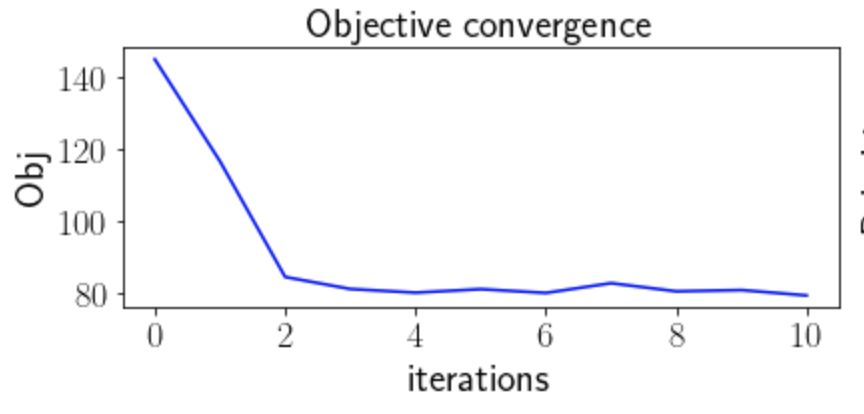
\includegraphics[height= 3cm, width=5cm]{figures/likelihood.png} \hspace{1cm} \\
  \vspace{0.5cm}
  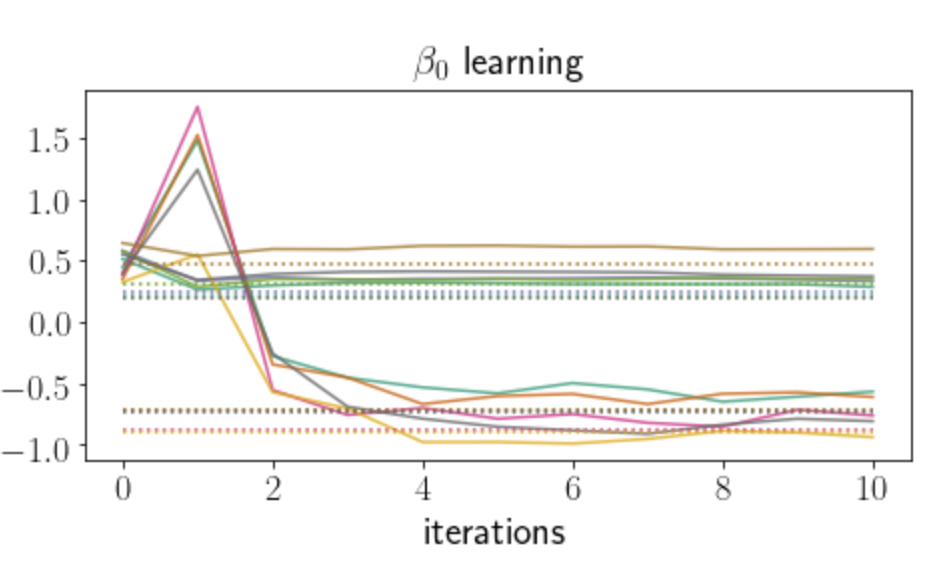
\includegraphics[height= 2cm, width=4cm]{figures/beta_learning.png} \hspace{0.7cm}
  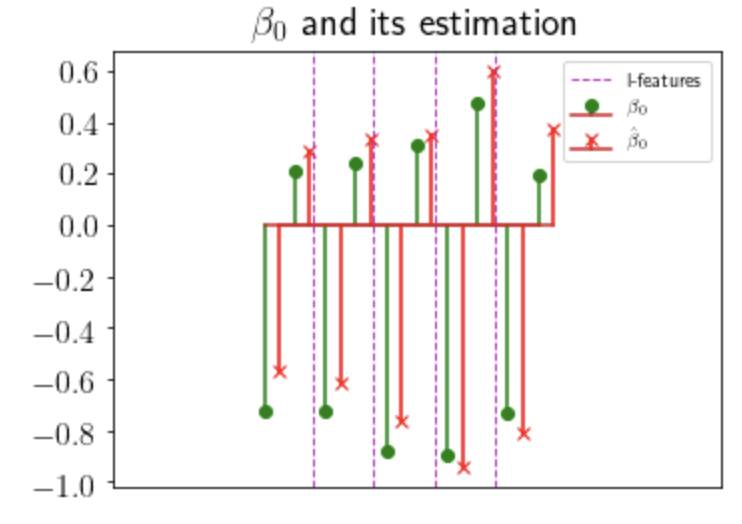
\includegraphics[height= 2cm, width=4cm]{figures/beta_estimation.png} \\
  \vspace{0.5cm}
  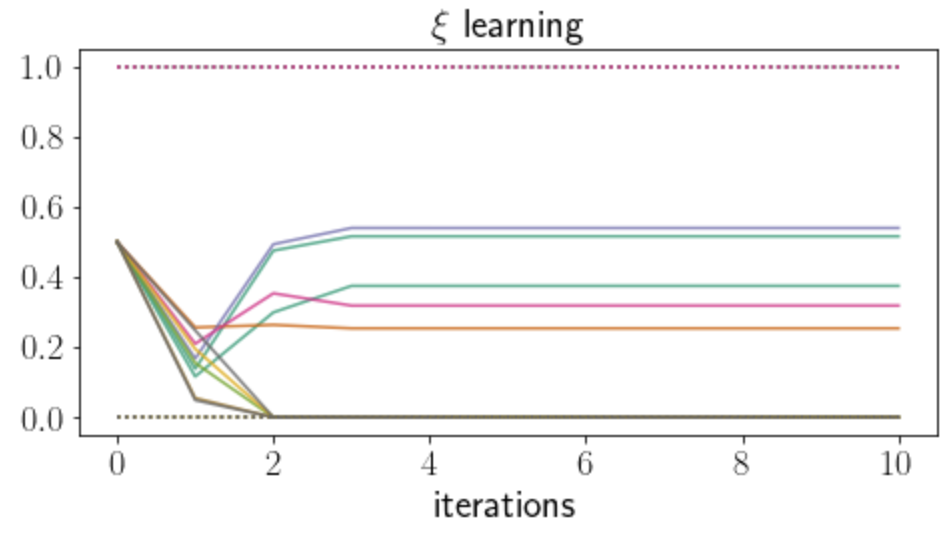
\includegraphics[height= 2cm, width=4cm]{figures/xi_learning.png} \hspace{0.7cm}
  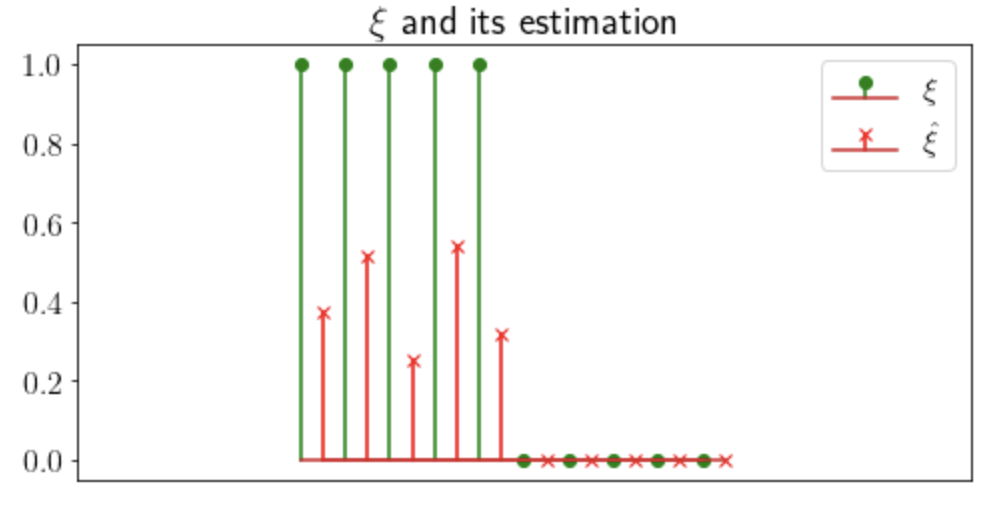
\includegraphics[height= 2cm, width=4cm]{figures/xi_estimation.png} \\
\end{frame}

\section{Conclusion}

\begin{frame}[noframenumbering]
\Large \centering
\textcolor{blue_pres}{VI.} Conclusion
\end{frame}

\begin{frame}{Conclusion}

\begin{itemize}
  \item Prognostic method called lights introduced to deal with the problem of joint modeling of longitudinal data and censored durations, where a large number of longitudinal features are available
  \item Penalization of the likelihood in order to perform feature selection and to prevent overfitting
  \item New efficient estimation algorithm (QNMCEM) has been derived
  \item Automatically determines significant prognostic longitudinal features
\end{itemize}

\begin{block}{\texttt{Python} 3 package}
\begin{itemize}
  \item Available at \small{\url{https://github.com/Califrais/lights}}
  \item Applications of the model available soon on an \texttt{arXiv} paper.
\end{itemize}
\end{block}

\end{frame}

\begin{frame}[noframenumbering]
\Large \centering
\textcolor{blue_pres}{} Thank you!
\end{frame}

\section{References}
\frame{
  \small
  \frametitle{References}
  \bibliographystyle{plainnat}
  \bibliography{refs}
}

\end{document}
              